\clearpage
\subsection{Expression} % (fold)
\label{sub:expression}

An Expression is a value used in a \nameref{sec:program-creation-statement}. These values may be calculated or entered directly into the source code of the Program.

\begin{figure}[h]
   \centering
   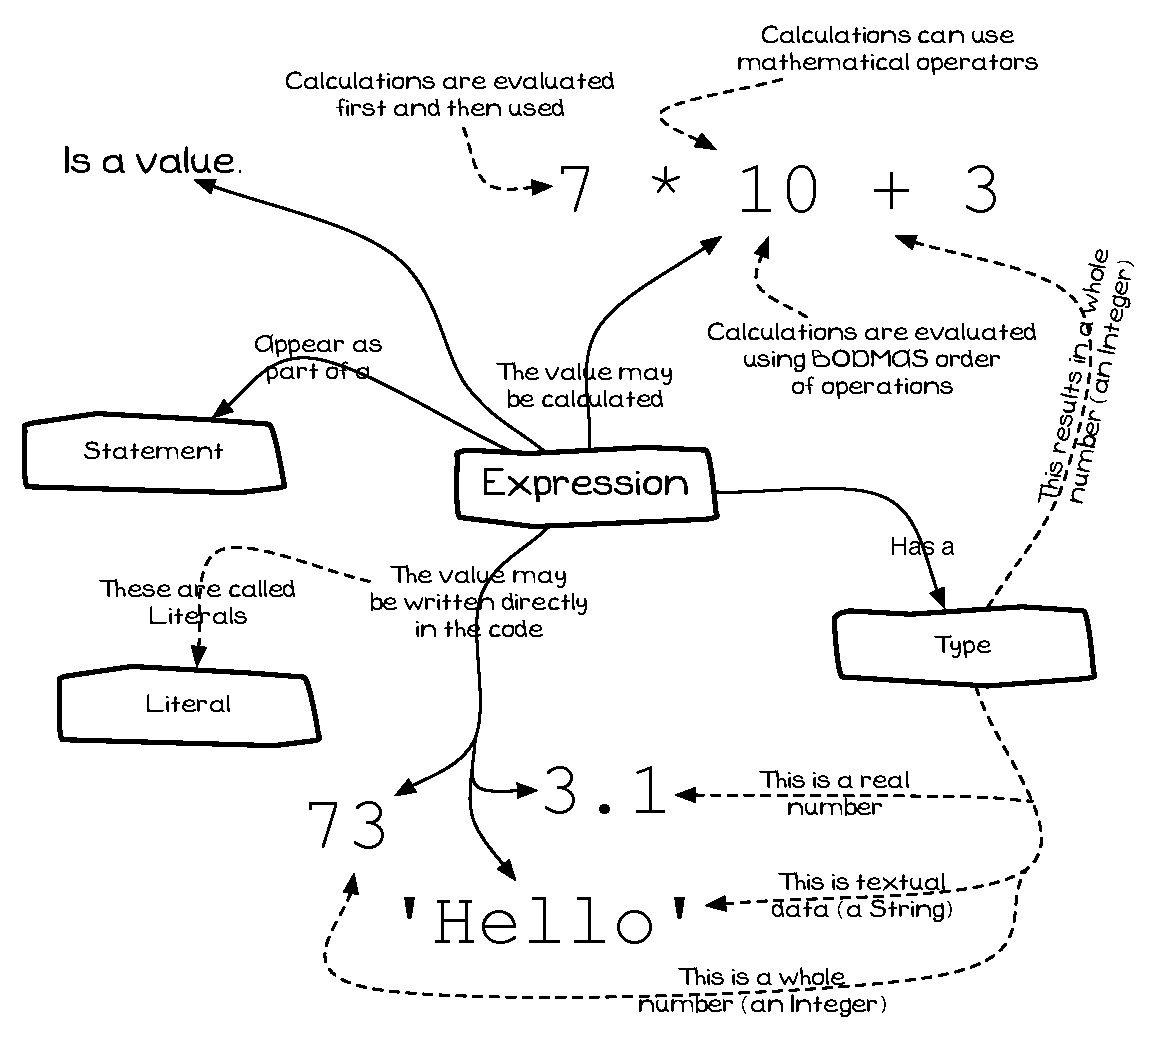
\includegraphics[width=\textwidth]{./topics/program-creation/diagrams/Expression} 
   \caption[Expression Concept Diagram]{An Expression provides a \textbf{value} to be used in a Statement.}
   \label{fig:program-creation-expression}
\end{figure}


\mynote{
\begin{itemize}
  \item The concepts related to Expressions are shown in Figure \ref{fig:program-creation-expression}.
  \item An Expression provides a \textbf{value} that is used in a Statement.
  \item The Expression's value may be calculated or entered directly into the code.
  \item Calculations can use mathematical operators: + for addition, - for subtraction, * for multiplication, $/$ for division, and parenthesis ( ) for grouping.
  \item Expressions are evaluated using the BODMAS order of operations.
  \item Values entered directly within an Expression are \textbf{Literal} values.
\end{itemize}
}

% section program (end)